\section{Systemarchitektur}
\setauthor{Elias Brandstätter}
Die Systemarchitektur des Health-Monitoring-Systems folgt einer mehrschichtigen Architektur, die aus einem Frontend, einem Backend sowie mehreren externen Datenquellen besteht. Ziel dieser Architektur ist es, Daten aus verschiedenen Plattformen zentral zu sammeln, zu analysieren und anschließend in einem übersichtlichen Dashboard darzustellen.

Durch die klare Trennung der einzelnen Komponenten wird eine modulare und wartbare Systemstruktur erreicht. Jede Schicht des Systems erfüllt eine spezifische Aufgabe und kommuniziert über definierte Schnittstellen mit den anderen Komponenten.


\subsection{Gesamtübersicht der Architektur}
\setauthor{Elias Brandstätter}
Das System besteht aus vier zentralen Ebenen:

\begin{compactitem}
    \item Frontend (Dashboard)
    \item Backend (API und Datenverarbeitung)
    \item Cloud- und Datenebene
    \item Externe Schnittstellen 
\end{compactitem}

Das Frontend dient als Benutzeroberfläche für Mitarbeiter des Unternehmens und ermöglicht die Anzeige sowie Analyse des Status aller Kunden-Apps. Das Backend stellt eine REST-API bereit, über die das Frontend Daten abrufen kann. Gleichzeitig übernimmt das Backend die Verarbeitung und Aggregation der Daten aus verschiedenen Quellen.

Die Cloud- und Datenebene stellt die zentrale Datenbasis dar, während externe Schnittstellen zusätzliche Informationen aus Drittplattformen liefern.


\subsection{Frontend-Schicht}
\setauthor{Zoe Emily Öllinger}
Das Frontend stellt die Benutzeroberfläche für die Mitarbeiter dar. Hier wird die Health-Übersicht und die Detailseite der einzelenen Apps dargestellt.

Das Frontend besteht aus:

\begin{compactitem}
    \item UI \& UX
    \item Health-Übersicht
    \item Detailseite
    \item Kommentar-Sektion
    \item Erkennung von Statusänderungen
\end{compactitem}


\subsection{Backend-Schicht}
\setauthor{Elias Brandstätter}
Das Backend stellt die zentrale Logik des Systems dar und fungiert als Vermittler zwischen Frontend, Datenbank und externen Schnittstellen. Die Backend-Komponente wurde mit FastAPI entwickelt und läuft auf dem ASGI-Server Uvicorn.

Die wichtigsten Aufgaben des Backends sind:

\begin{compactitem}
    \item Bereitstellung einer REST-API für das Frontend
    \item Abrufen und Verarbeiten von Daten aus Google BigQuery
    \item Integration externer APIs
    \item Durchführung von Statusanalysen
    \item Erkennung von Statusänderungen
\end{compactitem}

Das Backend aggregiert Daten aus mehreren Quellen und stellt sie in strukturierter Form bereit. Diese Daten werden anschließend vom Frontend dargestellt.

Ein wichtiger Bestandteil der Backend-Logik ist die Analyse der Statuswerte der einzelnen Apps. Hierbei werden verschiedene Health-Checks durchgeführt und deren Ergebnisse miteinander kombiniert, um einen Gesamtstatus zu bestimmen.

\subsection{Daten- und Cloud-Schicht}
\setauthor{Elias Brandstätter}
Die Datenbasis des Systems liegt in Google BigQuery, wo alle relevanten Monitoring-Daten gespeichert sind - darunter das aggregierte Health-Check-Label der jeweiligen Kunden-Apps, synchronisierte HubSpot-Ticket-Daten sowie App-Konfigurationsinformationen. Das Backend greift auf diese Daten ausschließlich über SQL-Abfragen zu, was eine präzise Datenextraktion ohne unnötigen Overhead ermöglicht.

Ergänzend dazu speichert das Backend täglich einen lokalen Snapshot des aktuellen Systemzustands als CSV-Datei. Diese Snapshots dienen als Vergleichsbasis für die automatische Erkennung von Statusänderungen, ohne dass eine eigene Historiendatenbank betrieben werden muss.

\subsection{Integration externer Systeme}
\setauthor{Elias Brandstätter}
Neben den eigenen Cloud-Ressourcen bindet das System zwei externe Plattformen ein, deren Daten das Bild über den Zustand einer Kunden-App vervollständigen. Asana liefert Informationen über offene Aufgaben, die einem Kunden zugeordnet sind, und ermöglicht das Erstellen neuer Tasks direkt aus dem Dashboard heraus. HubSpot stellt Support-Ticket-Daten bereit, die Aufschluss darüber geben, ob bereits aktive Supportfälle zu einer App existieren. Beide Datenquellen werden im Backend mit den BigQuery-Daten zusammengeführt und in einer einheitlichen Struktur an das Frontend übergeben.

\subsection{Datenfluss im System}
\setauthor{Elias Brandstätter}
Der typische Datenfluss lässt sich anhand des Aufrufs der Health-Check-Übersicht nachvollziehen:

\begin{enumerate}
\item Das Frontend sendet eine HTTP-Anfrage an den \texttt{/health-checks}-Endpunkt, optional ergänzt durch Filterparameter.
\item Das Backend führt an die BigQuery-Tabelle \texttt{health\_monitoring.health\_data} eine SQL-Abfrage aus und lädt parallel die aktuellen HubSpot-Ticketanzahlen sowie offene Asana-Tasks.
\item Die Daten aus allen Quellen werden pro Kunden-Slug zusammengeführt und mit dem zuletzt gespeicherten Snapshot verglichen, um Statusänderungen zu erkennen.
\item Das Backend gibt die aufbereiteten Daten als strukturiertes JSON-Objekt an das Frontend zurück, das die Ergebnisse im Dashboard darstellt.
\end{enumerate}


\section{UI und UX}
\setauthor{Zoe Emily Öllinger}
\subsection{UI und UX Design}
\setauthor{Zoe Emily Öllinger}

Das Design des Frontends wurde zu Beginn in Figma ausgearbeitet und weiters durch absprache und Feedback-Runden verbessert.

\subsubsection{Iteration 1:}
\setauthor{Zoe Emily Öllinger}

Im ersten Meeting mit der Firma wurden uns die Anforderungen für unsere Anwendung dargelegt und es wurde gebeten, zwei verschiedene Workflows zu entwickeln.
Dabei benötigen wir eine Übersichtsseite und eine Detailseite sowie einen Weg um zur Dokumentation in Confluence zu kommen und weiters eventuell auch Statistiken.

\subsubsection{Workflow-Version 1}
\setauthor{Zoe Emily Öllinger}

\begin{figure}[h]
    \centering
    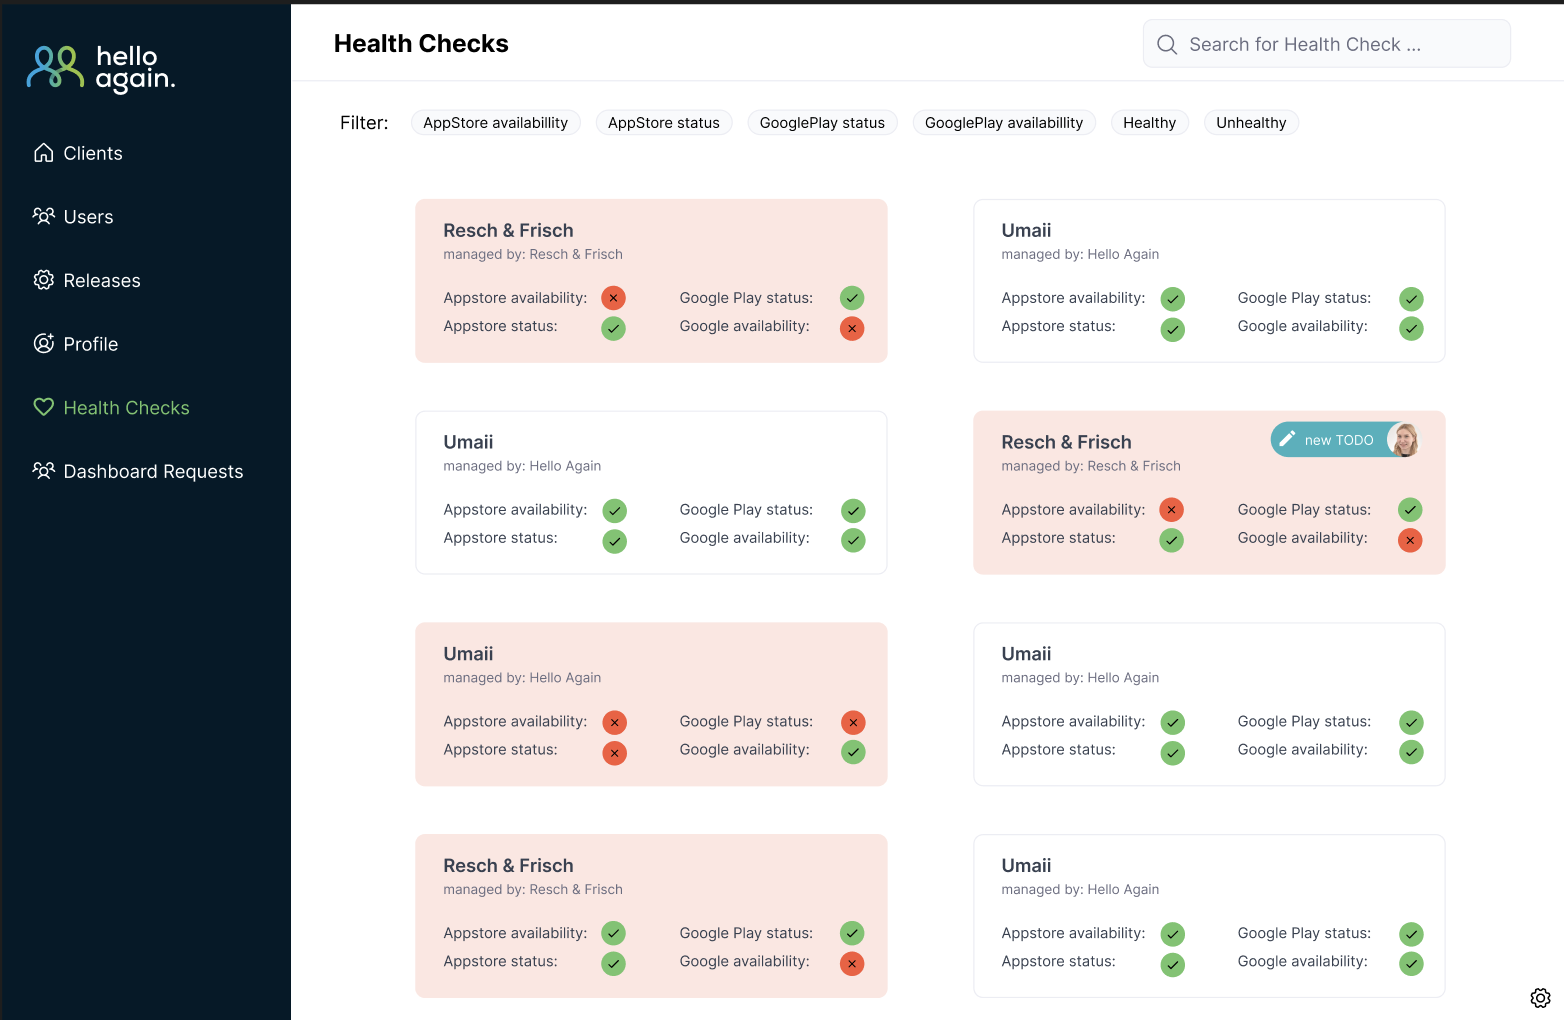
\includegraphics[width=0.8\textwidth]{pics/V1}
    \label{fig:version-1.1-des-dashboards}
\end{figure}

Dies ist die erste Version der Übersichtsseite.
Hier werden die verschiedenen Kunden angezeigt, sowie ein grober Überblick über die Health-Stati.
Je nach Farbe wird angezeigt ob die jeweiligen Apps Healthy oder Unhealthy sind (also ob sie Error werfen oder nicht).
Sobald eine App ausfällt wird sie sofort gekennzeichnet, damit die Mitarbeiter auch dementsprechend auf diese Ausfälle reagieren können.

\begin{figure}[h]
    \centering
    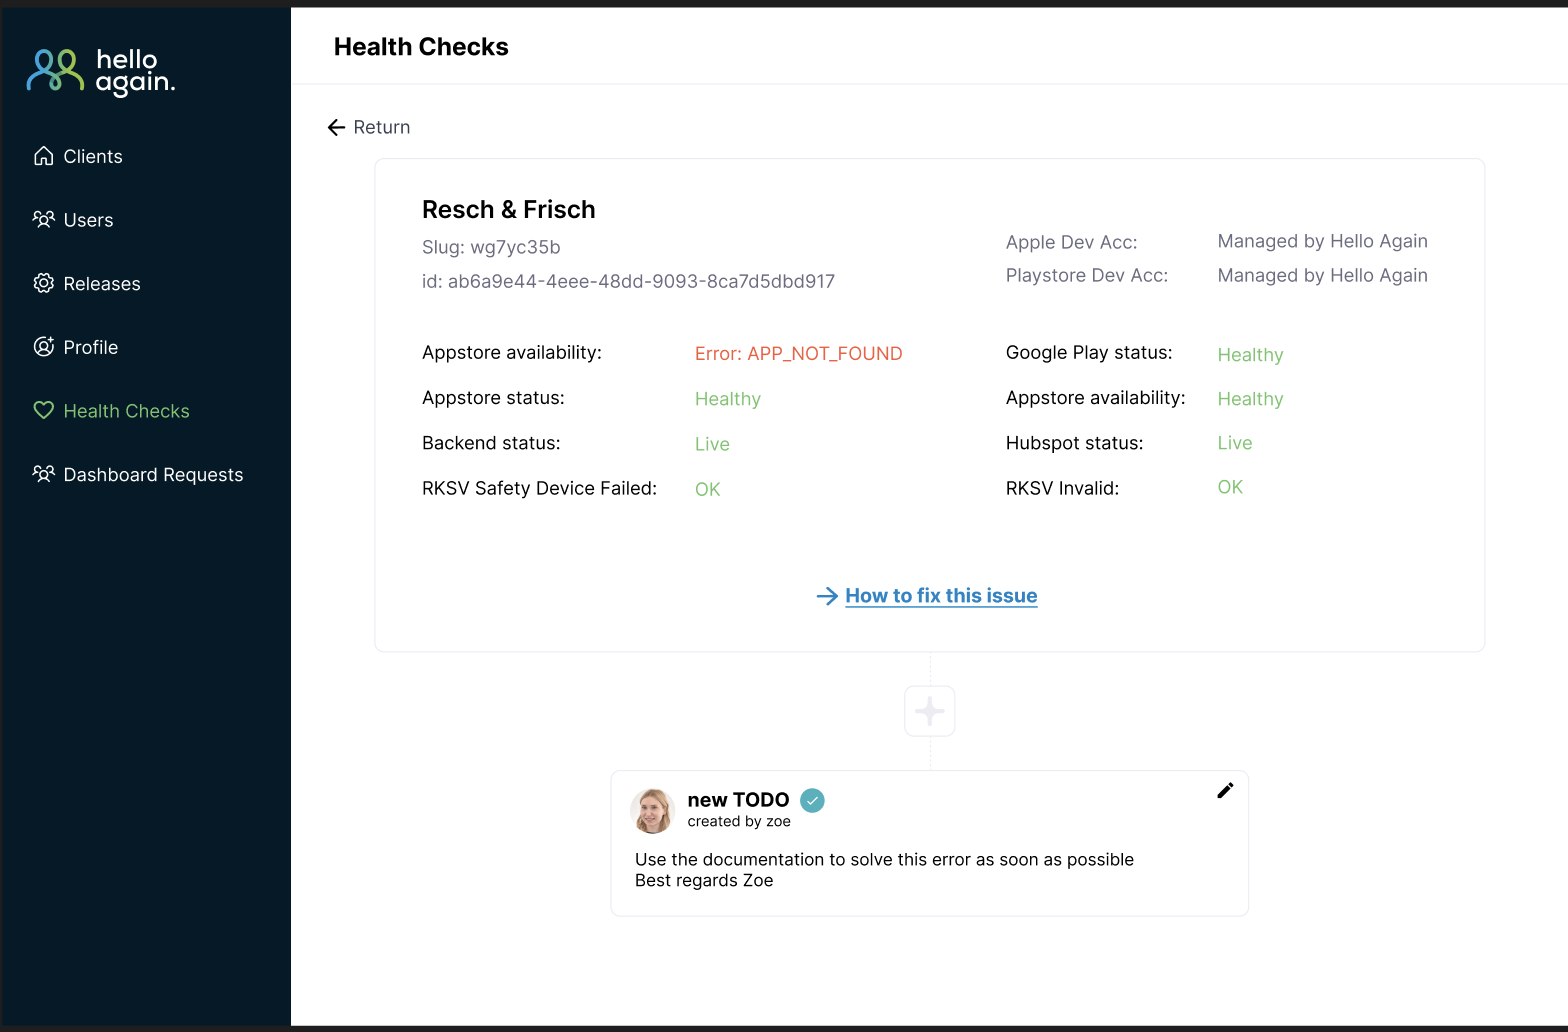
\includegraphics[width=0.8\textwidth]{pics/V2}
    \label{Version 1.2 des Dashboards}
\end{figure}

Dies ist die erste Version der Detailseite, auf der nochmal genauere Daten der Kunden angezeigt werden, sowie den Health-Status der einzelnen Health-Checks. Wird ein Fehler gemeldet wird auf der Detailsseite auch automatisch der Link angezeigt zur Lösung des Errors. Dies ermöglicht den Mitarbeitern eine effiziente und schnelle Arbeitsweise. Weiter unsen sehen wir noch eine TODO-Funktion. Hier kann man direkt im Dashboard Kommentare schreiben, die dann Plattformübergreifend in Asana erstellt werden.

\subsubsection{Workflow-Version 2}
\setauthor{Zoe Emily Öllinger}

\begin{figure}[h]
    \centering
    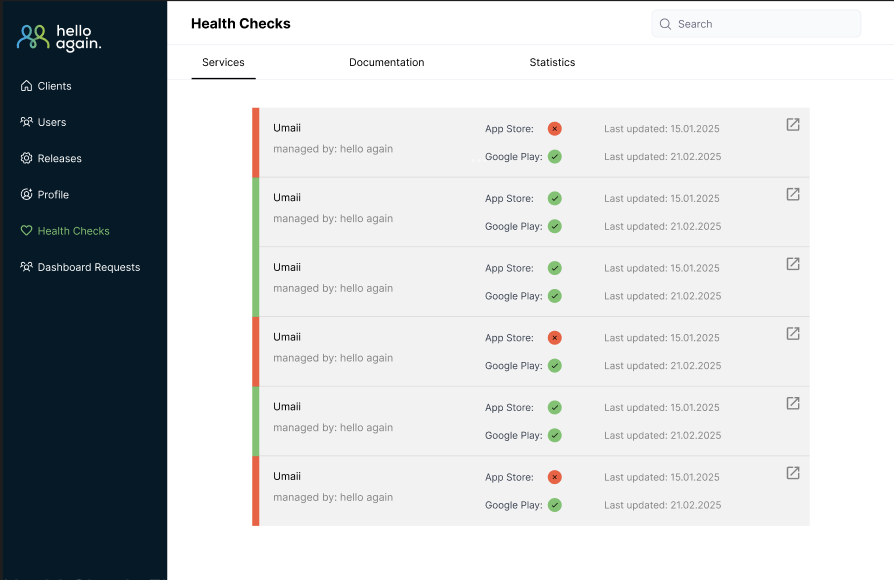
\includegraphics[width=0.8\textwidth]{pics/V3}
    \label{Version 2.1 des Dashboards}
\end{figure}

Dies ist die zweite Workflow-Version die erarbeitet wurde.
Hier haben wir ebenfalls eine Übersichtsseite mit einer Liste doch mit einem kleinen Unterschied.

\begin{figure}[h]
    \centering
    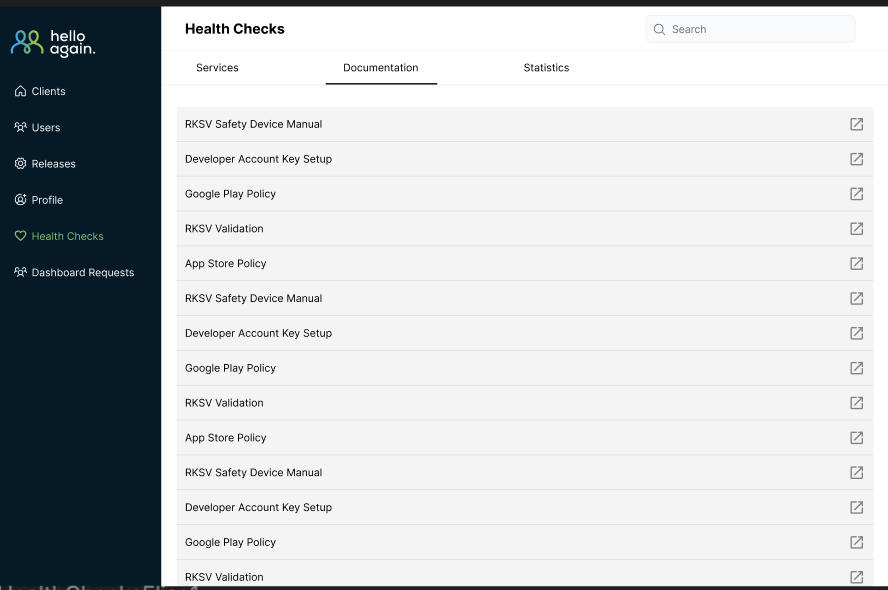
\includegraphics[width=0.8\textwidth]{pics/V4}
    \label{fig:version-2.2-des-dashboards}
\end{figure}

Um zu Dokumentationsseite zu gelangen kann der Tab gewechselt werden, allerdings werden hier alle vorhandenen Dokumentationen zur Fehlerbehebung angezeigt.

\begin{figure}[h]
    \centering
    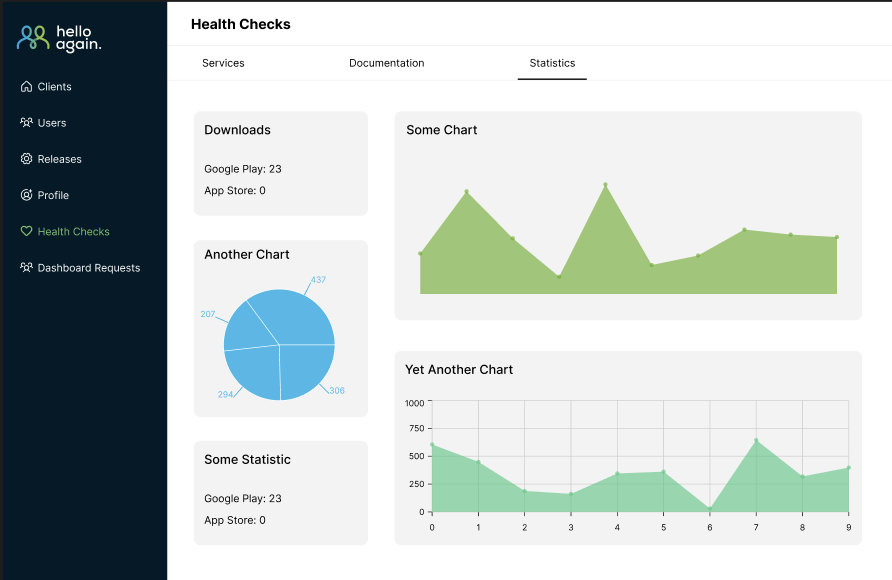
\includegraphics[width=0.8\textwidth]{pics/V5}
    \label{Version 2.3 des Dashboards}
\end{figure}

Als dritten Tab wurde eine Statistik-Übersicht eingebaut bei der man die Downloads der letzten Tage sieht, sowie die Anzahl der App-Ausfälle, damit man potenzielle Fehlerquellen zeitnahe erkennen und beseitigen kann.

\begin{figure}[h]
    \centering
    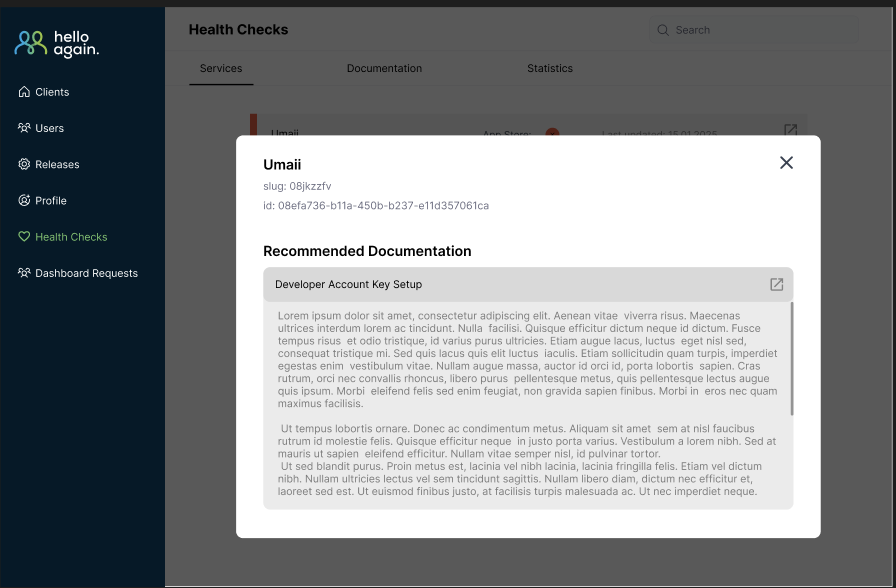
\includegraphics[width=0.8\textwidth]{pics/V7}
    \label{Version 2.4 des Dashboards}
\end{figure}

Die Detailseite sieht sehr ähnlich aus zum ersten Workflow-Konzept allerdings mit dem Unterschied, dass man die Detailseite als Popup sieht.
Unten rechts erscheint ein Button mit dem Namen Resolve Errors.
Klickt man auf diesen, wird ein Fenster angezeigt, dass uns die Dokumentation zur Fehlerbehebung liefert.

\subsubsection{Iteration 2:}
\setauthor{Zoe Emily Öllinger}

Zur Vorstellung beider Konzepte wurden wir in die Firma eingeladen und haben diese dort auch Vorgestellt.
Es wurde schnell klar, dass wir eine Übersichtsseite sowie eine Detailseite brauchen würden mit einer erweiterten Kommentarfunktion und einem Link zur externen Fehlerbehebung, darum wurde sich auf eine Misch-Version der beiden Workflows geeinigt.
Allerdings musste die Liste aller Kunden auf der Übersichtsseite noch etwas schmaler und informativer werden.

\begin{figure}[h]
    \centering
    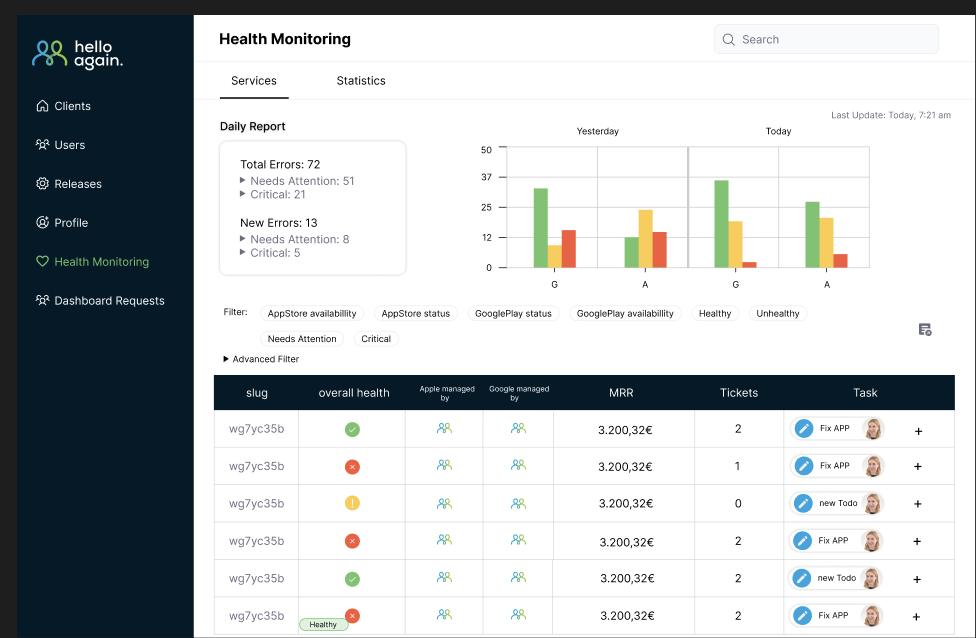
\includegraphics[width=0.8\textwidth]{pics/V9}
    \label{Version 3.1 des Dashboards}
\end{figure}

Hier sehen wir das verbesserte Dashboard-Design, dass nach dem ersten Feedback-Gespräch zustande kam.
Es wurde eine Übersichtliche Statistik eingearbeitet sowie eine schmalere Liste mit mehr nützlichen Informationen für die Mitarbeiter.
Dazu wurden noch Quickfilter eingebaut, die ermöglichen sollen, dass man schnell alle fehlerhaften Apps herausfiltern kann, damit die Zeit, die die App nicht im Appstore verfügbar ist, so klein wie möglich gehalten wird, um so wenig potenziellen Umsatz wie möglich zu verlieren.
Dazu gibt es noch die Advanced-Filter Option.
Diese ist dafür da um nach konkreten Fehlern filtern zu können.
Wenn man zum Beispiel weiß, dass das Liscenseagreement von Google geändert wurde, kann man mit den Advanced-Filtern danach suchen und diese Fehler beheben.
Beim Overall-Health-Status wurde noch eine dritte Option eingführt neben Healthy und Healthy.
Diese heißt Needs-Attention, dass heißt die App könnte bald aus dem Appstore oder Googleplaystore entfernt werden, da Lizenzen abgelaufen sind.
Auch ein Schnellzugriff auf die TODOS soll gewährleistet sein.

\begin{figure}[h]
    \centering
    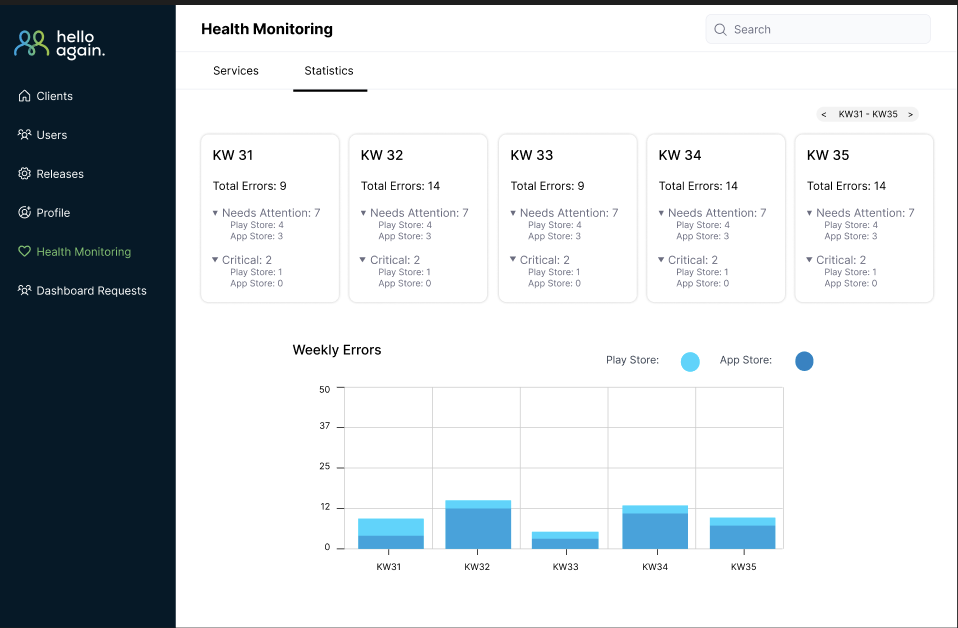
\includegraphics[width=0.8\textwidth]{pics/V8}
    \label{Version 3.2 des Dashboards}
\end{figure}

Weiters gibt es einen eigenen Tab, der die Statistiken auf der Übersichtsseite nochmals erweitert und mit mehr Informationen darstellt.

\begin{figure}[h]
    \centering
    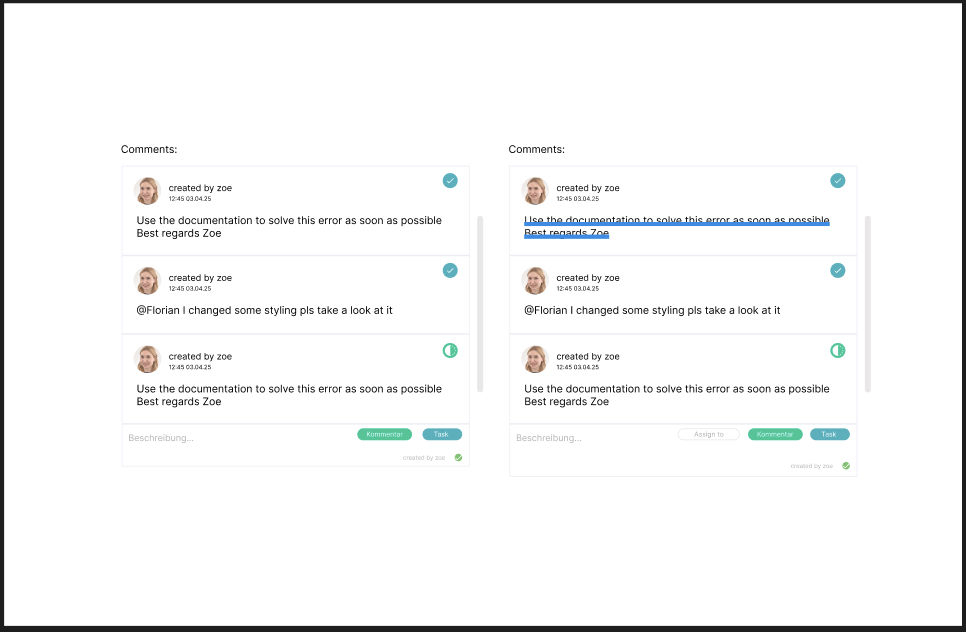
\includegraphics[width=0.8\textwidth]{pics/V12}
    \label{Version 3.3 des Dashboards}
\end{figure}

Dazu wurde die Kommentar- und TODO-Funktion nochmals überarbeitet in zwei verschiednen Version, hier wurde sich schlussendlich für diese Version (siehe Bild oben) entschieden.


\section{Dashboard}
\setauthor{Zoe Emily Öllinger}
\subsection{Übersichtsseite}
\setauthor{Zoe Emily Öllinger}

\subsubsection{Tabellenansicht}
\setauthor{Zoe Emily Öllinger}

Zu Beginn wurde die Tabelle erstellt auf der Übersichtsseite, hier werden die wichtigsten Daten der Kunden, für die Mitarbeiter dargestellt.
Man muss beachten, dass das Design der finalen Version des Dashboards von der Figma Version abweicht, da die Firma intern Code guidelines hat, an die wir uns halten mussten.
Ebenfalls gab es styling Guidelines und Komponenten die uns zu Verfügung gestellt wurden, wie zum Beispiel die Pagination.

\begin{figure}[h]
    \centering
    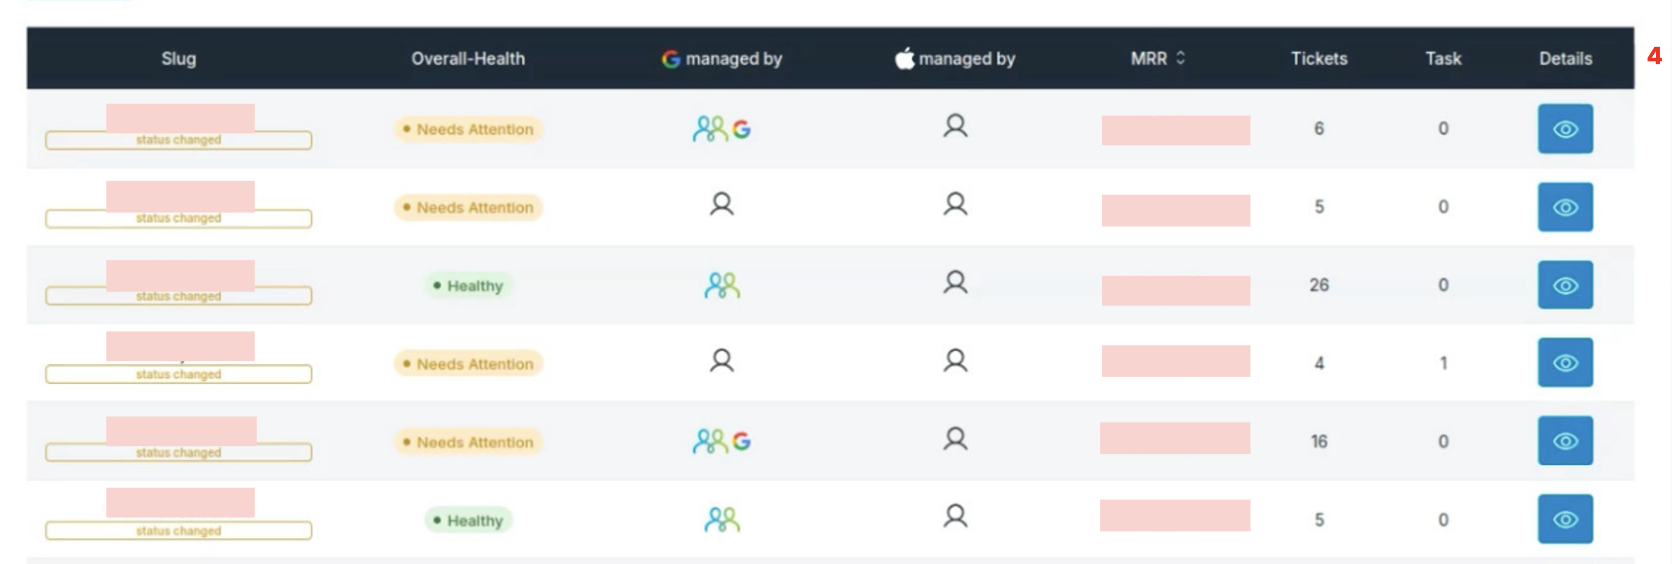
\includegraphics[width=0.8\textwidth]{pics/P4}
    \label{fig:Dashboard-Tabelle}
    \caption{Dashboard-Tabelle}
\end{figure}

Hier werden angezeigt:
\begin{compactitem}
\item der Slug (Eindeutiger Kundenbezeichner; zeigt auch ein status changed-Tag, falls sich der Status geändert hat)
\item Overall-Health (Ampelstatus des Clients (Healthy, Needs Attention, Unhealthy, Critical))
\item Google managed by (Zuständiges Team/Person für den Google-Account)
\item Apple managed by (Zuständiges Team/Person für den Apple-Kanal)
\item MRR (Monthly Recurring Revenue)
\item Tickets (Anzahl offener Support-Tickets)
\item Task (Anzahl offener Aufgaben)
\item Details (Link zur Detailseite)
\end{compactitem}

Da die Tabelle das Herzstück des Dashboards ist wurde sie als erstes implementiert und alles andere darauf aufgebaut.
Bei der Tabelle wurde auch daraus geachtet, dass die Columns filterbar sind nach dem höchsten oder niedrigsten MRR.

\subsubsection{Suchfunktion}
\setauthor{Zoe Emily Öllinger}

\begin{figure}[h]
    \centering
    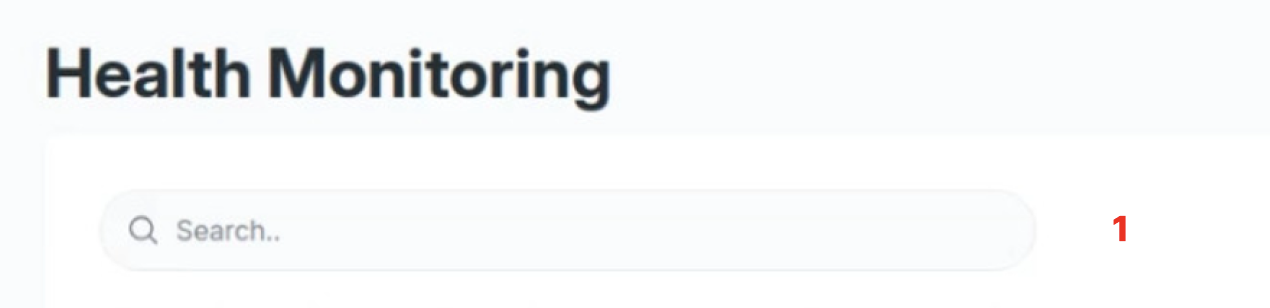
\includegraphics[width=0.8\textwidth]{pics/P1}
    \label{fig:Suchfunktion}
    \caption{Suchfunktion}
\end{figure}

Als nächstes wurde eine Suchfunktion implementiert, bei der man nach dem Slug filtern kann.
Die Suchfunktion ist hierbei caseinsensitive.

\subsubsection{Quickfilter}
\setauthor{Zoe Emily Öllinger}

\begin{figure}[h]
    \centering
    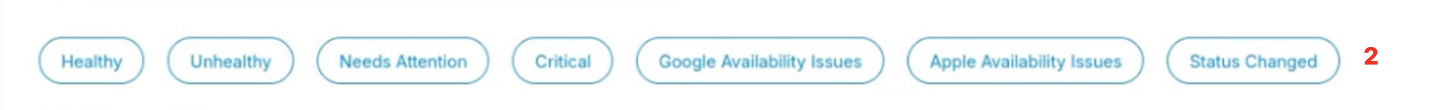
\includegraphics[width=0.8\textwidth]{pics/P2}
    \label{fig:Quickfilter}
    \caption{Quickfilter}
\end{figure}

Um den Mitarbeitern eine möglichst schnelle Filteroption zu bieten, gibt es die Quickfilter, diese sind als multiselect implementiert worden.
Das heißt man kann zum Beispiel nach allen Apps filtern, die unhealthy sind und mit status changed geflagged sind.
Das bedeutet, die App war gestern noch auf Healthy oder Needs Attention und ist heute aus den Stores geflogen.

Was bedeuten die Quickfilter Optionen?
\begin{compactitem}
    \item Healthy (Die App weist keine Fehler auf)
    \item Needs Attention (Die App wird bald aus den Stores entfernt)
    \item Critical (Die App wurde aus den Stores entfernt und ist nichtmehr verfügbar)
    \item Unhealthy (Der Status der App ist entweder Needs Attention oder Critical. Hier muss etwas getan werden!)
    \item Google Availability Issues (Der Google Playstore weist Probleme bei der App auf)
    \item Apple Availability Issues (Der Appstore weist Probleme bei der App auf)
    \item Status Changed (Der Status hat sich zum Vortag verändert)
\end{compactitem}

Das Filtern wird hier vom Frontend übernommen, da wir alle Daten der Tabelle benötigen und diese schon in das Frontend geladen haben.
Würden wir wieder eine Request an das Backend schicken, würden wir unnötig Zeit des Benutzers verschwenden.

\subsubsection{Advanced Filter}
\setauthor{Zoe Emily Öllinger}

\begin{figure}[h]
    \centering
    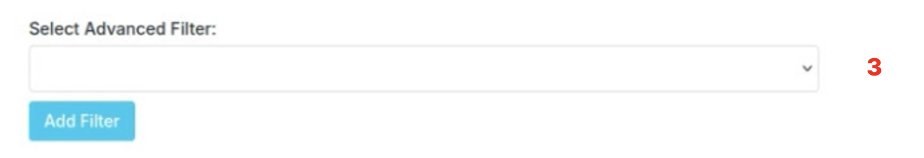
\includegraphics[width=0.8\textwidth]{pics/P3}
    \label{fig:AdvancedFilter}
    \caption{AdvancedFilter}
\end{figure}

Die Advanced Filter wurden erst zum Schluss implementiert, da diese Filteroption durch das Backend passiert.
Wir bekommen alle vorhandenen Fehler die vorkommen vom Backend ins Frontend und diese werden als zweiteilige Filteroption dargestellt.
Zuerst wählt man aus nach was man Filtern möchte zum Beispiel Google Availability und danach muss man auswählen welchen spezifischen Error Code man ansehen möchte.
Hier auch wieder ein Beispiel man hat Google Availability ausgewählt mit dem spezifischen Error Code License Agreement ran out.
Das Frontend hat keinen Zugriff auf die Error Codes der einzelenen Apps, daher wird eine Anfrage an das Backend geschickt mit dem Error Code nachdem gefiltert werden soll.
Anschließend wird die Liste neu gefiltert.
Da wir eine sehr große menge an Daten durchgehen müssen, dauert dieser Vorgang auch dementsprechend lange.

\subsubsection{Finale Version der Übersichtsseite}
\begin{figure}[h]
    \centering
    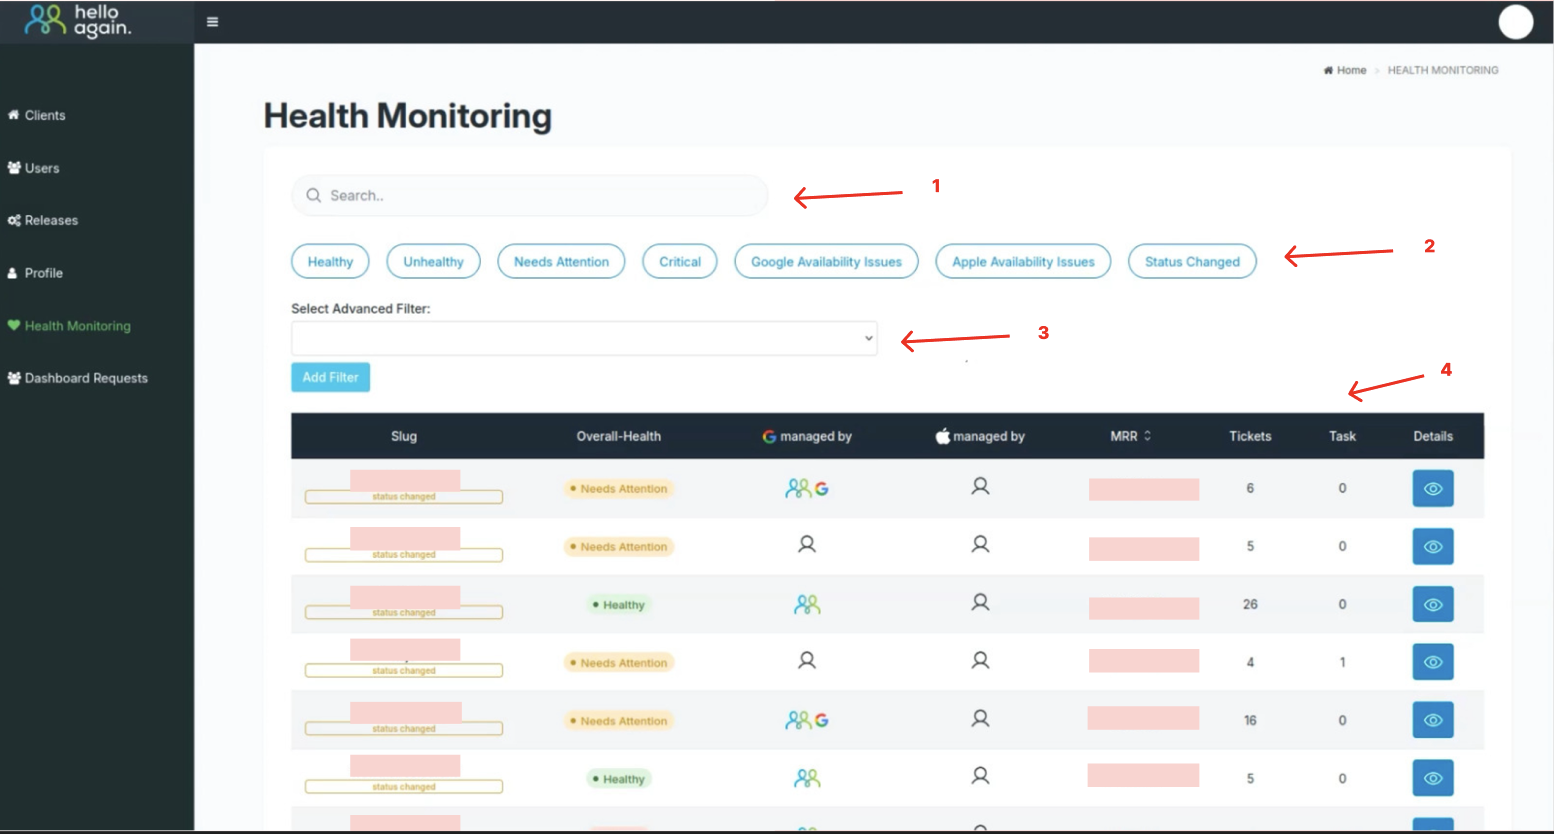
\includegraphics[width=0.8\textwidth]{pics/P5}
    \label{fig:Uebersichtsseite}
    \caption{Übersichtsseite}
\end{figure}
\clearpage
\subsection{Detailseite}
\setauthor{Zoe Emily Öllinger}

\subsubsection{Status Changed}
\setauthor{Zoe Emily Öllinger}

\begin{figure}[h]
    \centering
    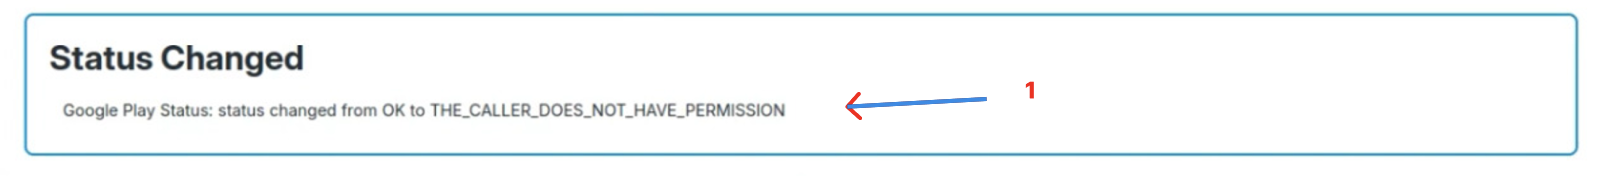
\includegraphics[width=0.8\textwidth]{pics/P8}
    \label{fig:StatusChanged}
    \caption{Status Changed}
\end{figure}

Am Anfang der Detailseite befindet sich die Status-Changed Flag.
Dieser wird nochmal visuell hervorgehoben und zeigt an wie sich die App im gegensatz zum Vortag verändert hat.
Sollte die App den Status von Healthy zu Unhealthy verändern wird der Error Code, der für diesen Fehler verantwortlich ist auch angezeigt.
Somit weiß der Benutzer sofort wo das Problem liegt.
Status Changed wird allerdings auch angezeigt, wenn die App sich von Unhealthy zu Healthy ändert, so können die Mitarbeiter zum Beispiel nach der App, die gestern noch Fehlerhaft war suchen und sehen auf den ersten Blick, ob sich ihr Status verändert hat.
Die Status changed Flags werden hier über eine Fetch-Request ins Frontend geladen.

\subsubsection{General Data}
\setauthor{Zoe Emily Öllinger}

\begin{figure}[h]
    \centering
    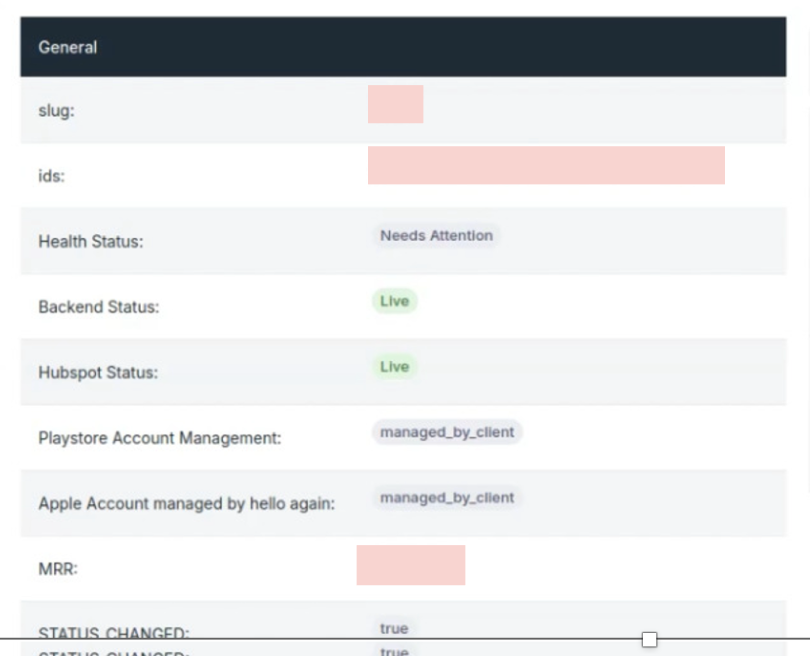
\includegraphics[width=0.8\textwidth]{pics/P9}
    \label{fig:GeneralData}
    \caption{General Data}
\end{figure}

Unter dem Status Changed Flag werden nochmals generelle Daten der App angezeigt, die auf der Übersichtsseite schon einsehbar sind.
Hier wurde darauf geachtet, dass die Daten jederzeit erweiterbar sind.
Das heißt, wenn wir aus dem Backend ergänzend noch YRR Daten bekommen würden, würde das Frontend sie ohne fremdeinwirkung eines Entwicklers darstellen.

\subsubsection{Kommentar Sektion}
\setauthor{Zoe Emily Öllinger}

\begin{figure}[h]
    \centering
    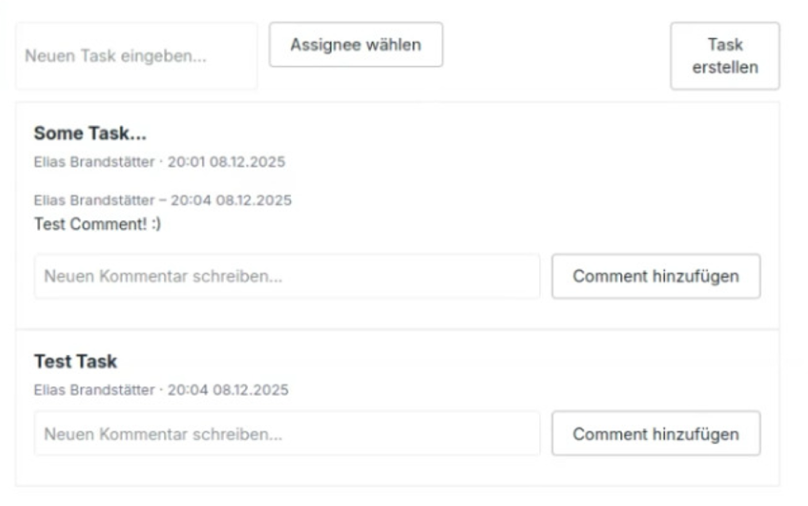
\includegraphics[width=0.8\textwidth]{pics/P10}
    \label{fig:KommentarSektion}
    \caption{Kommentarsektion}
\end{figure}

Die Kommentarsektion ist eine der wichtigsten Funktionen der Detailsseite.
Hier können Kommentare und Tasks erstellt werden, die ebenso in Asana erstellt werden.
Ebenso werden die Kommentare und Tasks, die bereits in Asana vorhanden sind dargstellt.
Wenn man einen Task erstellt kann man auch noch einen Assignee wählen, dem dieser Task dann zugeteilt wird.
Hierzu bekommen wir aus dem Backend alle Namen der Mitarbeiter, die auf dieses Asana Board Zugriff haben.
Wenn wir einen Task erstellen, wird der Text, der Slug und der Name des Assignees an das Backend übergeben, dass dan anschließend den Task in Asana erstellt.

\subsubsection{Health-Checks}
\setauthor{Zoe Emily Öllinger}

\begin{figure}[h]
    \centering
    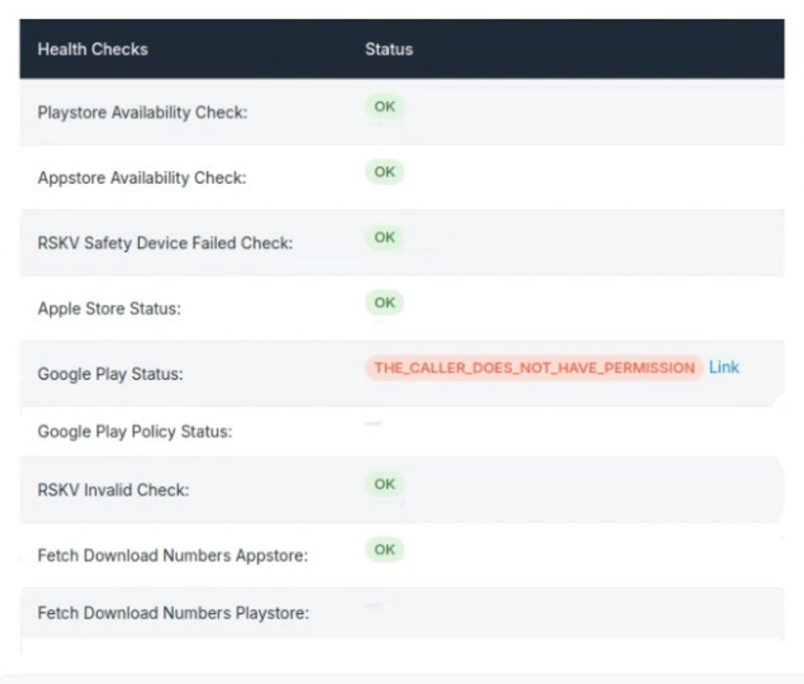
\includegraphics[width=0.8\textwidth]{pics/P11}
    \label{fig:Health-Checks}
    \caption{Health-Checks}
\end{figure}
\clearpage

Eine weitere wichtige Funktion der Detailseite sind die Health-Checks.
Hier wird der Status farblich gekennzeichnet, dass man sofort erkennt welche App Probleme wirft.
Wenn ein Error vorliegt wird immer dessen Fehlermeldung angezeigt, sowie ein Link zu Fehlerbehebung.
Drückt man auf den link wird man zur passenden Fehlerbeheungsdokumentation oder Anleitung in Confluence weitergeleitet.
Diese Health-Checks sowie die passenden Links der Doku werden vom Backend bereitgestellt.


\subsubsection{Tasks und Tickets}
\setauthor{Zoe Emily Öllinger}

\begin{figure}[h]
    \centering
    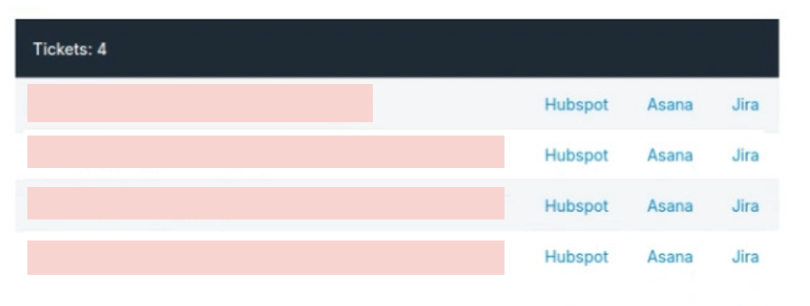
\includegraphics[width=0.8\textwidth]{pics/P12}
    \label{fig:TasksundTickets}
    \caption{Tasks und Tickets}
\end{figure}

Es wurde außerdem gewünscht, dass die Tasks und Tickets dargestellt werden, da alle 3 miteinander intern verlinkt sind.
Daher wird der Text beziehungsweise die Beschreibung der jeweils offenen Tickets angezeigt und die Links zur jeweiligen Plattform.
Wichtig ist zu betonen, dass hier nur offenene Tickets dargestellt werden.

\subsubsection{Finale Version der Detailsseite}
\setauthor{Zoe Emily Öllinger}

\begin{figure}[h]
    \centering
    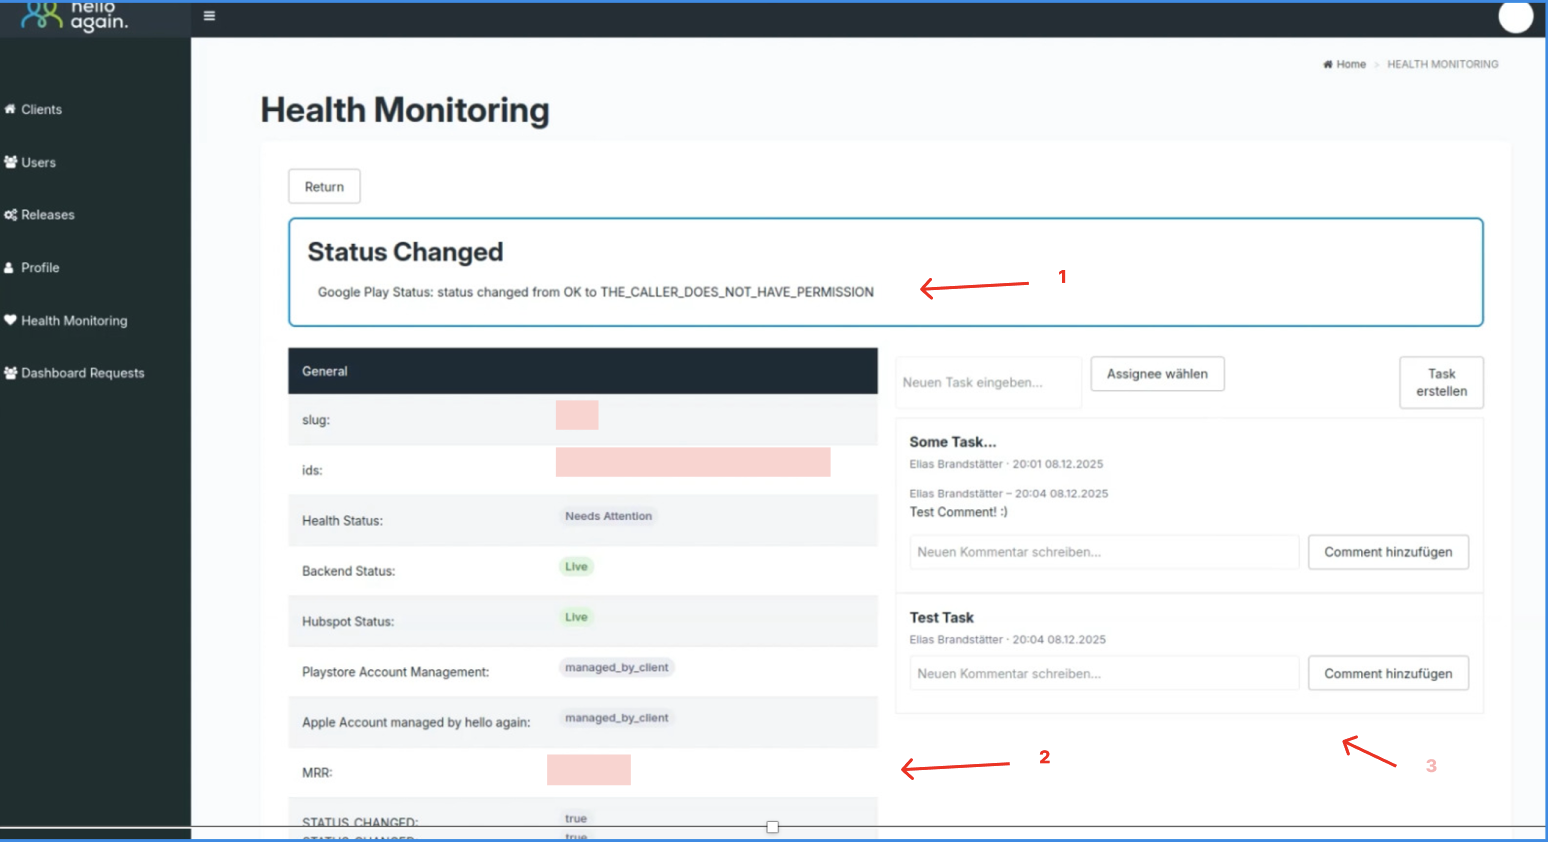
\includegraphics[width=0.8\textwidth]{pics/P6}
    \label{fig:FinaleVersionDetailseite1}
    \caption{Finale Version Detailseite 1}
\end{figure}

\begin{figure}[h]
    \centering
    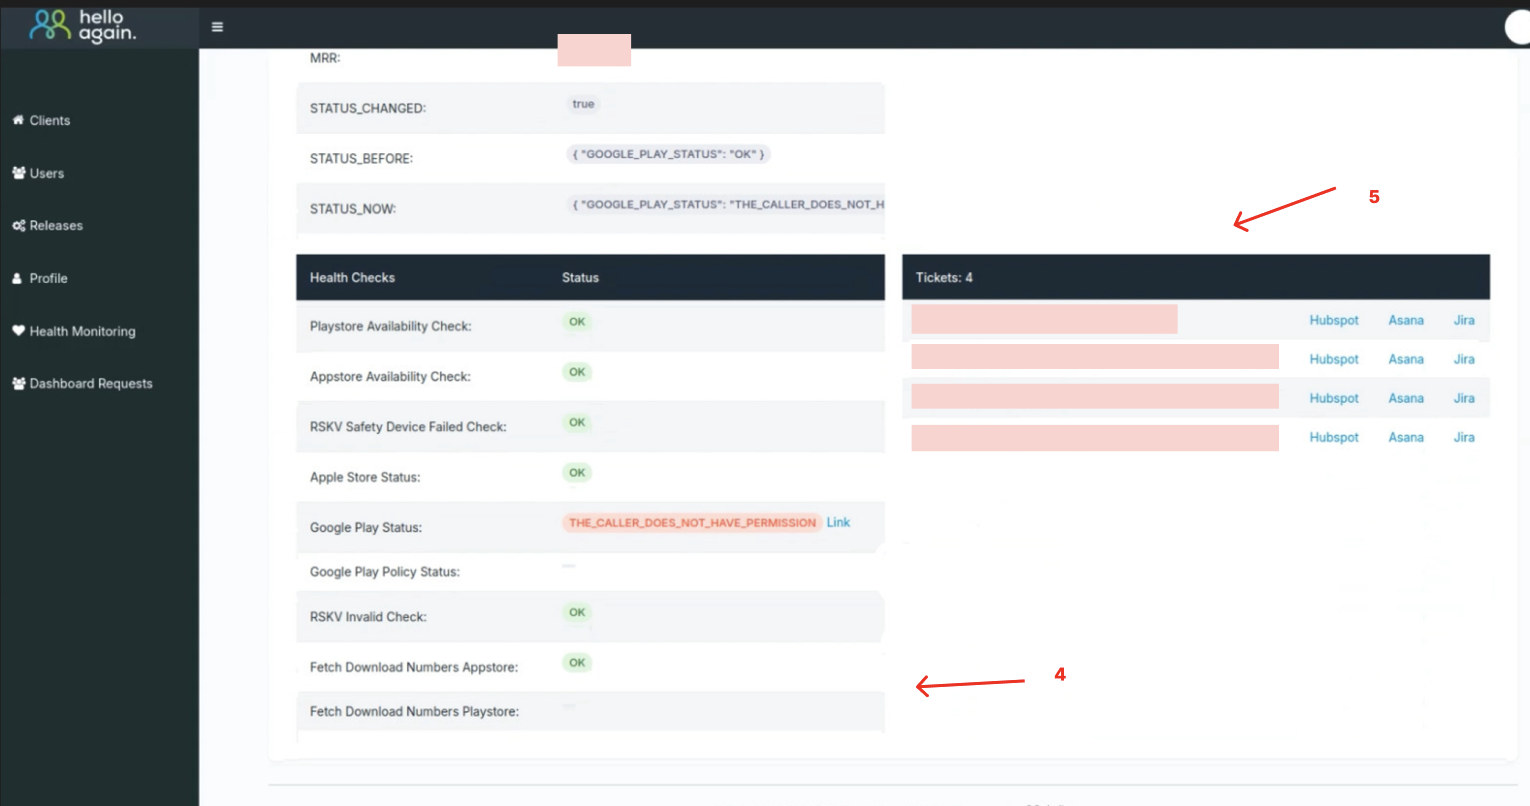
\includegraphics[width=0.8\textwidth]{pics/P7}
    \label{fig:FinaleVersionDetailseite2}
    \caption{Finale Version Detailseite 2}
\end{figure}



\section{Backend-Implementierung}
\setauthor{Elias Brandstätter}



\section{Integration externer Systeme}
\setauthor{Elias Brandstätter}



\section{Datenmanagement}
\setauthor{Elias Brandstätter}



\section{Fehlerbehandlung und Logging}
\setauthor{Elias Brandstätter}



\section{Sicherheit und Zugriff}
\setauthor{Zoe Emily Öllinger}
\subsection{Einleitung}
\setauthor{Zoe Emily Öllinger}

Im Rahmen unserer Diplomarbeit bei Hello Again wurde dem Thema Sicherheit und Datenschutz von Beginn an ein hoher Stellenwert gegeben.
Bereits zu Beginn der Diplomarbeit fand eine Einschulung statt, in der uns die Richtlinien zum sicheren Umgang mit Daten, Systemen und Tools erklärt wurden.
Diese Richtlinien betrafen sowohl den Umgang mit sensiblen Kundendaten als auch die erlaubten Tools.

\subsection{Datenschutz und der Umgang mit Kundendaten}
\setauthor{Zoe Emily Öllinger}

Einer der wichtigsten Punkte betraf den Umgang mit Kundendaten.
Uns wurde explizit erklärt, dass Kundendaten zu keinem Zeitpunkt in externe KI-Systeme eingegeben werden dürfen.
Konkret wurde dabei ChatGPT als Beispiel genannt; ein öffentliches KI-Tool, das von OpenAI betrieben wird.
Kundendaten unterliegen in der Europäischen Union der Datenschutz-Grundverordnung (DSGVO), die strenge Anforderungen an die Verarbeitung, Speicherung und Weitergabe personenbezogener Daten stellt.
Werden diese Daten an Dienste weitergegeben, ohne dass eine entsprechende rechtliche Grundlage vorliegt, ist dies ein Datenschutzverstoß, der für das Unternehmen erhebliche rechtliche und finanzielle Konsequenzen haben kann.
Das Vertrauen der Kunden in die Plattform von Hello Again sehr wichtig; jede Form von Databreach würde das Vertrauen beschädigen zwischen Kunde und Firma.
Für uns heißt das, dass wir darauf achten mussten, bei der Nutzung von KI-Tools ausschließlich selbst erstellte Beispieldaten zu verwenden.
Keine echten Kundendaten!


\subsection{Erlaubte KI-Tools: Firmeninterne Lösungen}
\setauthor{Zoe Emily Öllinger}

Hello Again setzt auf firmenintern verwaltete KI-Lösungen.
Im Rahmen der Diplomarbeit durften waren zwei Tools zur Nutzung freigegeben.
Google Gemini (bezahlte Firmenversion): Hello Again verwendet die kostenpflichtige, unternehmensseitig verwaltete Version von Google Gemini.
Der Unterschied zur kostenlosen öffentlichen Version ist, dass Google mit Enterprise-Verträgen garantiert, dass die Daten nicht für das Training von Modellen zu verwendet werden.
Claude als Konsolentool (bezahlte Version im Firmen-Environment): Zusätzlich duften wir Claude von Anthropic verwenden, jedoch ausschließlich in der bezahlten Version.
Claude wurde dabei als Konsolentool eingesetzt, also für Debugging-Unterstützung.

Hier kann man erkennen, dass die Unternehmen die neuartigen KI-Tools nicht ablehnen sondern ihre Mitarbeiter ermutigen diese sinnvoll einzusetzen.


\subsection{Sensibilisierung für Phishing-Angriffe}

Ein weiterer Bestandteil der Einschulung war die Aufklärung über Phishing-Angriffe.
Phishing bezeichnet den Versuch, Mitarbeiter durch gefälschte E-Mails, Links oder Webseiten dazu zu bringen, sensible Informationen herauszugeben zum Beispiel Passwörter, Zugangsdaten uvm.
Für Unternehmen sind Phishing-Angriffe besonders gefährlich, weil sie häufig gezielt auf bestimmte Organisationen abgezielt sind.
Wir wurden gebeten, bei jeder E-Mail mit unbekanntem Absender oder ungewöhnlichem Inhalt besonders Vorsicht zu sein, keine Links einfach so zu öffnen und Rücksprache mit unserem Betreuer zu halten.

\subsection{Branches}
Wir arbeiteten nicht direkt auf dem Main Branch des Projekts.
Der Main Branch enthält den Code der das Dashboard am laufen hält.
Direkte Änderungen an diesem Branch würden ein Risiko darstellen, da fehlerhafte Commits Auswirkungen auf das laufende Dashboard haben könnten bzw haben.
Stattdessen wurde uns ein Branch namens health-monitoring bereitgestellt.
Dieser Branch war unser main Arbeitsbereich.
Er war vom Main Branch isoliert, sodass unsere Änderungen restliche Projekt nicht beeinflussen konnten.
Innerhalb unseres health-monitoring-Branches legten wir uns zwei weitere Branches an, um eine klare Trennung zwischen Frontend und Backend zu gewährleisten, einen frontend-Branch für alle Arbeiten an UI und UX, sowie einen backend-Branch für die serverseitige Logik, API-Anbindungen und Datenbankoperationen.
So konnten effizient Merge-Konflikte reduziert werden.
Am Ende der Diplomarbeit wurde unser erarbeiteter Code nach der Überprüfung, durch die Devs in das offizielle Projekt gemerged.

\subsection{Kein separates Mockup-Projekt}

In vielen Firmen ist es üblich, Praktikanten oder Schülerinnen und Schülern ein Demoprojekt zur Verfügung zu stellen, an dem sie arbeiten können.
In unserem Fall war dies firmenintern nicht machbar.
Der Grund war personeller und zeitlicher Aufwand.
Das Aufsetzen eines Mockup-Projekts hätte viel Zeit und Entwickler gekostet.
Da diese Devs nicht verfügbar waren, entschied man sich für einen eigenen Branch.
Diese Entscheidung hatte sowohl Vorteile als auch Nachteile.
Der offensichtliche Vorteil liegt darin, dass wir mit echten firmeninternen Strukturen gearbeitet haben aber der Nachteil besteht darin, dass die Fehlertoleranz geringer ist.
Schwerwiegende Fehler im Branch hätten den Merge-Prozess erschwert.
Da aber die Entwickler unsere Commits regelmäßig begutachtet haben, hatten wir diese Probleme nicht.












































% beispiel materials zum verwenden
%\begin{table}
%    \centering
%    \begin{tabular}{|lcc|}
%    \hline
%              & \textbf{Regular Customers} & \textbf{Random Customers} \\ \hline
%    Age       & 20-40                      & \textgreater{}60          \\ \hline
%    Education & university                 & high school               \\ \hline
%    \end{tabular}
%    \caption{Ein paar tabellarische Daten}
%    \label{tab:impl:data}
%\end{table}
%
%\begin{figure}
%    \centering
%    \includegraphics[scale=0.5]{pics/knuthi.jpg}
%    \caption{Don Knuth -- CS Allfather}
%    \label{fig:impl:knuth}
%\end{figure}
%
%Siehe und staune in Abb. \ref{fig:impl:knuth}.
%\lipsum[6-9]
%Dann betrachte den Code in Listing \ref{lst:impl:foo}.
%
%\begin{lstlisting}[language=Python,caption=Some code,label=lst:impl:foo]
%# Program to find the sum of all numbers stored in a list (the not-Pythonic-way)
%
%# List of numbers
%numbers = [6, 5, 3, 8, 4, 2, 5, 4, 11]
%
%# variable to store the sum
%sum = 0
%
%# iterate over the list
%for val in numbers:
%    sum = sum+val
%
%print("The sum is", sum)
%\end{lstlisting}